\documentclass[12pt]{beamer}\usepackage[]{graphicx}\usepackage[]{color}
%% maxwidth is the original width if it is less than linewidth
%% otherwise use linewidth (to make sure the graphics do not exceed the margin)
\makeatletter
\def\maxwidth{ %
  \ifdim\Gin@nat@width>\linewidth
    \linewidth
  \else
    \Gin@nat@width
  \fi
}
\makeatother

\definecolor{fgcolor}{rgb}{0.345, 0.345, 0.345}
\newcommand{\hlnum}[1]{\textcolor[rgb]{0.686,0.059,0.569}{#1}}%
\newcommand{\hlstr}[1]{\textcolor[rgb]{0.192,0.494,0.8}{#1}}%
\newcommand{\hlcom}[1]{\textcolor[rgb]{0.678,0.584,0.686}{\textit{#1}}}%
\newcommand{\hlopt}[1]{\textcolor[rgb]{0,0,0}{#1}}%
\newcommand{\hlstd}[1]{\textcolor[rgb]{0.345,0.345,0.345}{#1}}%
\newcommand{\hlkwa}[1]{\textcolor[rgb]{0.161,0.373,0.58}{\textbf{#1}}}%
\newcommand{\hlkwb}[1]{\textcolor[rgb]{0.69,0.353,0.396}{#1}}%
\newcommand{\hlkwc}[1]{\textcolor[rgb]{0.333,0.667,0.333}{#1}}%
\newcommand{\hlkwd}[1]{\textcolor[rgb]{0.737,0.353,0.396}{\textbf{#1}}}%

\usepackage{framed}
\makeatletter
\newenvironment{kframe}{%
 \def\at@end@of@kframe{}%
 \ifinner\ifhmode%
  \def\at@end@of@kframe{\end{minipage}}%
  \begin{minipage}{\columnwidth}%
 \fi\fi%
 \def\FrameCommand##1{\hskip\@totalleftmargin \hskip-\fboxsep
 \colorbox{shadecolor}{##1}\hskip-\fboxsep
     % There is no \\@totalrightmargin, so:
     \hskip-\linewidth \hskip-\@totalleftmargin \hskip\columnwidth}%
 \MakeFramed {\advance\hsize-\width
   \@totalleftmargin\z@ \linewidth\hsize
   \@setminipage}}%
 {\par\unskip\endMakeFramed%
 \at@end@of@kframe}
\makeatother

\definecolor{shadecolor}{rgb}{.97, .97, .97}
\definecolor{messagecolor}{rgb}{0, 0, 0}
\definecolor{warningcolor}{rgb}{1, 0, 1}
\definecolor{errorcolor}{rgb}{1, 0, 0}
\newenvironment{knitrout}{}{} % an empty environment to be redefined in TeX

\usepackage{alltt}
\usepackage{graphicx}
\usepackage{tikz}
\setbeameroption{hide notes}
\setbeamertemplate{note page}[plain]
\usepackage{listings}

% get rid of junk
\usetheme{default}
\usefonttheme[onlymath]{serif}
\beamertemplatenavigationsymbolsempty
\hypersetup{pdfpagemode=UseNone} % don't show bookmarks on initial view

% named colors
\definecolor{offwhite}{RGB}{255,250,240}
\definecolor{gray}{RGB}{155,155,155}

\ifx\notescolors\undefined % slides

  \definecolor{foreground}{RGB}{80,80,80}
  \definecolor{background}{RGB}{255,255,255}
  \definecolor{title}{RGB}{255,199,0}
  \definecolor{subtitle}{RGB}{89,132,212}
  \definecolor{hilit}{RGB}{248,117,79}
  \definecolor{vhilit}{RGB}{255,111,207}
  \definecolor{lolit}{RGB}{200,200,200}
  \definecolor{lit}{RGB}{255,199,0}
  \definecolor{mdlit}{RGB}{89,132,212}
  \definecolor{link}{RGB}{248,117,79}

\else % notes
  \definecolor{background}{RGB}{255,255,255}
  \definecolor{foreground}{RGB}{24,24,24}
  \definecolor{title}{RGB}{27,94,134}
  \definecolor{subtitle}{RGB}{22,175,124}
  \definecolor{hilit}{RGB}{122,0,128}
  \definecolor{vhilit}{RGB}{255,0,128}
  \definecolor{lolit}{RGB}{95,95,95}
\fi
\definecolor{nhilit}{RGB}{128,0,128}  % hilit color in notes
\definecolor{nvhilit}{RGB}{255,0,128} % vhilit for notes

\newcommand{\hilit}{\color{hilit}}
\newcommand{\vhilit}{\color{vhilit}}
\newcommand{\nhilit}{\color{nhilit}}
\newcommand{\nvhilit}{\color{nvhilit}}
\newcommand{\lit}{\color{lit}}
\newcommand{\mdlit}{\color{mdlit}}
\newcommand{\lolit}{\color{lolit}}

% use those colors
\setbeamercolor{titlelike}{fg=title}
\setbeamercolor{subtitle}{fg=subtitle}
\setbeamercolor{frametitle}{fg=gray}
\setbeamercolor{structure}{fg=subtitle}
\setbeamercolor{institute}{fg=lolit}
\setbeamercolor{normal text}{fg=foreground,bg=background}
%\setbeamercolor{item}{fg=foreground} % color of bullets
%\setbeamercolor{subitem}{fg=hilit}
%\setbeamercolor{itemize/enumerate subbody}{fg=lolit}
\setbeamertemplate{itemize subitem}{{\textendash}}
\setbeamerfont{itemize/enumerate subbody}{size=\footnotesize}
\setbeamerfont{itemize/enumerate subitem}{size=\footnotesize}

% center title of slides
\setbeamertemplate{blocks}[rounded]
\setbeamertemplate{frametitle}[default][center]
% margins
\setbeamersize{text margin left=25pt,text margin right=25pt}

% page number
\setbeamertemplate{footline}{%
    \raisebox{5pt}{\makebox[\paperwidth]{\hfill\makebox[20pt]{\lolit
          \scriptsize\insertframenumber}}}\hspace*{5pt}}

% add a bit of space at the top of the notes page
\addtobeamertemplate{note page}{\setlength{\parskip}{12pt}}

% default link color
\hypersetup{colorlinks, urlcolor={link}}

\ifx\notescolors\undefined % slides
  % set up listing environment
  \lstset{language=bash,
          basicstyle=\ttfamily\scriptsize,
          frame=single,
          commentstyle=,
          backgroundcolor=\color{darkgray},
          showspaces=false,
          showstringspaces=false
          }
\else % notes
  \lstset{language=bash,
          basicstyle=\ttfamily\scriptsize,
          frame=single,
          commentstyle=,
          backgroundcolor=\color{offwhite},
          showspaces=false,
          showstringspaces=false
          }
\fi

% a few macros
\newcommand{\code}[1]{\texttt{#1}}
\newcommand{\hicode}[1]{{\hilit \texttt{#1}}}
\newcommand{\bb}[1]{\begin{block}{#1}}
\newcommand{\eb}{\end{block}}
\newcommand{\bi}{\begin{itemize}}
%\newcommand{\bbi}{\vspace{24pt} \begin{itemize} \itemsep8pt}
\newcommand{\bbi}{\vspace{4pt} \begin{itemize} \itemsep8pt}
\newcommand{\ei}{\end{itemize}}
\newcommand{\bv}{\begin{verbatim}}
\newcommand{\ev}{\end{verbatim}}
\newcommand{\ig}{\includegraphics}
\newcommand{\subt}[1]{{\footnotesize \color{subtitle} {#1}}}
\newcommand{\ttsm}{\tt \small}
\newcommand{\ttfn}{\tt \footnotesize}
\newcommand{\figh}[2]{\centerline{\includegraphics[height=#2\textheight]{#1}}}
\newcommand{\figw}[2]{\centerline{\includegraphics[width=#2\textwidth]{#1}}}



%------------------------------------------------
% end of header
%------------------------------------------------

\title{Introduction to Data Visualization}
\subtitle{STAT 133}
\author{\href{http://www.gastonsanchez.com}{Gaston Sanchez}}
\institute{Department of Statistics, UC{\textendash}Berkeley}
\date{\href{http://www.gastonsanchez.com}{\tt \scriptsize \color{foreground} gastonsanchez.com}
\\[-4pt]
\href{http://github.com/gastonstat/stat133}{\tt \scriptsize \color{foreground} github.com/gastonstat/stat133}
\\[-4pt]
{\scriptsize Course web: \href{http://www.gastonsanchez.com/stat133}{\tt gastonsanchez.com/stat133}}
}
\IfFileExists{upquote.sty}{\usepackage{upquote}}{}
\begin{document}


{
  \setbeamertemplate{footline}{} % no page number here
  \frame{
    \titlepage
  } 
}

%------------------------------------------------

\begin{frame}
\begin{center}
\Huge{\hilit{Graphics}}
\end{center}
\end{frame}

%------------------------------------------------

\begin{frame}
\frametitle{Data Visualization}

Using only numerical reduction methods in data analyses is far too limiting

\end{frame}

%------------------------------------------------

\begin{frame}[fragile]
\frametitle{Motivation}

Consider some data (four pairs of variables)
\begin{knitrout}\footnotesize
\definecolor{shadecolor}{rgb}{0.969, 0.969, 0.969}\color{fgcolor}\begin{kframe}
\begin{verbatim}
##     x1     y1  x2    y2  x3     y3  x4     y4
## 1   10   8.04  10  9.14  10   7.46   8   6.58
## 2    8   6.95   8  8.14   8   6.77   8   5.76
## 3   13   7.58  13  8.74  13  12.74   8   7.71
## 4    9   8.81   9  8.77   9   7.11   8   8.84
## 5   11   8.33  11  9.26  11   7.81   8   8.47
## 6   14   9.96  14  8.10  14   8.84   8   7.04
## 7    6   7.24   6  6.13   6   6.08   8   5.25
## 8    4   4.26   4  3.10   4   5.39  19  12.50
## 9   12  10.84  12  9.13  12   8.15   8   5.56
## 10   7   4.82   7  7.26   7   6.42   8   7.91
## 11   5   5.68   5  4.74   5   5.73   8   6.89
\end{verbatim}
\end{kframe}
\end{knitrout}

\end{frame}

%------------------------------------------------

\begin{frame}
\begin{center}
\large{\mdlit{What things would you like \\ to calculate for each variable?}}
\end{center}
\end{frame}

%------------------------------------------------

\begin{frame}[fragile]
\frametitle{Motivation}

\begin{knitrout}\scriptsize
\definecolor{shadecolor}{rgb}{0.969, 0.969, 0.969}\color{fgcolor}\begin{kframe}
\begin{verbatim}
##        x1             x2             x3             x4    
##  Min.   : 4.0   Min.   : 4.0   Min.   : 4.0   Min.   : 8  
##  1st Qu.: 6.5   1st Qu.: 6.5   1st Qu.: 6.5   1st Qu.: 8  
##  Median : 9.0   Median : 9.0   Median : 9.0   Median : 8  
##  Mean   : 9.0   Mean   : 9.0   Mean   : 9.0   Mean   : 9  
##  3rd Qu.:11.5   3rd Qu.:11.5   3rd Qu.:11.5   3rd Qu.: 8  
##  Max.   :14.0   Max.   :14.0   Max.   :14.0   Max.   :19
\end{verbatim}
\end{kframe}
\end{knitrout}

\begin{knitrout}\scriptsize
\definecolor{shadecolor}{rgb}{0.969, 0.969, 0.969}\color{fgcolor}\begin{kframe}
\begin{verbatim}
##        y1               y2              y3              y4        
##  Min.   : 4.260   Min.   :3.100   Min.   : 5.39   Min.   : 5.250  
##  1st Qu.: 6.315   1st Qu.:6.695   1st Qu.: 6.25   1st Qu.: 6.170  
##  Median : 7.580   Median :8.140   Median : 7.11   Median : 7.040  
##  Mean   : 7.501   Mean   :7.501   Mean   : 7.50   Mean   : 7.501  
##  3rd Qu.: 8.570   3rd Qu.:8.950   3rd Qu.: 7.98   3rd Qu.: 8.190  
##  Max.   :10.840   Max.   :9.260   Max.   :12.74   Max.   :12.500
\end{verbatim}
\end{kframe}
\end{knitrout}

\end{frame}

%------------------------------------------------

\begin{frame}
\begin{center}
\large{\mdlit{What things would you like to calculate \\ for each pair of variables (e.g. \code{x1, y1})?}}
\end{center}
\end{frame}

%------------------------------------------------

\begin{frame}[fragile]
\frametitle{Motivation}

\begin{knitrout}\footnotesize
\definecolor{shadecolor}{rgb}{0.969, 0.969, 0.969}\color{fgcolor}\begin{kframe}
\begin{alltt}
\hlkwd{cor}\hlstd{(anscombe}\hlopt{$}\hlstd{x1, anscombe}\hlopt{$}\hlstd{y1)}
\end{alltt}
\begin{verbatim}
## [1] 0.8164205
\end{verbatim}
\begin{alltt}
\hlkwd{cor}\hlstd{(anscombe}\hlopt{$}\hlstd{x2, anscombe}\hlopt{$}\hlstd{y2)}
\end{alltt}
\begin{verbatim}
## [1] 0.8162365
\end{verbatim}
\begin{alltt}
\hlkwd{cor}\hlstd{(anscombe}\hlopt{$}\hlstd{x3, anscombe}\hlopt{$}\hlstd{y3)}
\end{alltt}
\begin{verbatim}
## [1] 0.8162867
\end{verbatim}
\begin{alltt}
\hlkwd{cor}\hlstd{(anscombe}\hlopt{$}\hlstd{x4, anscombe}\hlopt{$}\hlstd{y4)}
\end{alltt}
\begin{verbatim}
## [1] 0.8165214
\end{verbatim}
\end{kframe}
\end{knitrout}

\end{frame}

%------------------------------------------------

\begin{frame}[fragile]
\frametitle{Motivation}

\bi
  \item Mean of \code{x} values = 9.0
  \item Mean of \code{y} values = 7.5
  \item least squares equation: $y = 3 + 0.5x$
  \item Sum of squared errors: 110
  \item Correlation coefficient: 0.816
\ei

\end{frame}

%------------------------------------------------

\begin{frame}[fragile]
\frametitle{Why Graphics?}

Are you able to see any patterns, associations, relations?
\begin{knitrout}\scriptsize
\definecolor{shadecolor}{rgb}{0.969, 0.969, 0.969}\color{fgcolor}\begin{kframe}
\begin{verbatim}
##     x1     y1  x2    y2  x3     y3  x4     y4
## 1   10   8.04  10  9.14  10   7.46   8   6.58
## 2    8   6.95   8  8.14   8   6.77   8   5.76
## 3   13   7.58  13  8.74  13  12.74   8   7.71
## 4    9   8.81   9  8.77   9   7.11   8   8.84
## 5   11   8.33  11  9.26  11   7.81   8   8.47
## 6   14   9.96  14  8.10  14   8.84   8   7.04
## 7    6   7.24   6  6.13   6   6.08   8   5.25
## 8    4   4.26   4  3.10   4   5.39  19  12.50
## 9   12  10.84  12  9.13  12   8.15   8   5.56
## 10   7   4.82   7  7.26   7   6.42   8   7.91
## 11   5   5.68   5  4.74   5   5.73   8   6.89
\end{verbatim}
\end{kframe}
\end{knitrout}

{\small Famous dataset \code{"anscombe"} (four data sets)}
\end{frame}

%------------------------------------------------

\begin{frame}[fragile]
\frametitle{Why Graphics?}

How are these two variables associated?

\bigskip
What does these data values look like?
\begin{knitrout}\scriptsize
\definecolor{shadecolor}{rgb}{0.969, 0.969, 0.969}\color{fgcolor}\begin{kframe}
\begin{verbatim}
##     x1     y1
## 1   10   8.04
## 2    8   6.95
## 3   13   7.58
## 4    9   8.81
## 5   11   8.33
## 6   14   9.96
## 7    6   7.24
## 8    4   4.26
## 9   12  10.84
## 10   7   4.82
## 11   5   5.68
\end{verbatim}
\end{kframe}
\end{knitrout}

\end{frame}

%------------------------------------------------

\begin{frame}
\begin{center}
\large{
\mdlit{Our eyes are not very good at making sense when looking at (many) numbers}
\pause

\bigskip
\hilit{But they are great for looking at shapes and detecting patterns}
}
\end{center}
\end{frame}

%------------------------------------------------

\begin{frame}[fragile]
\frametitle{Why Graphics}

\begin{knitrout}\footnotesize
\definecolor{shadecolor}{rgb}{0.969, 0.969, 0.969}\color{fgcolor}

{\centering 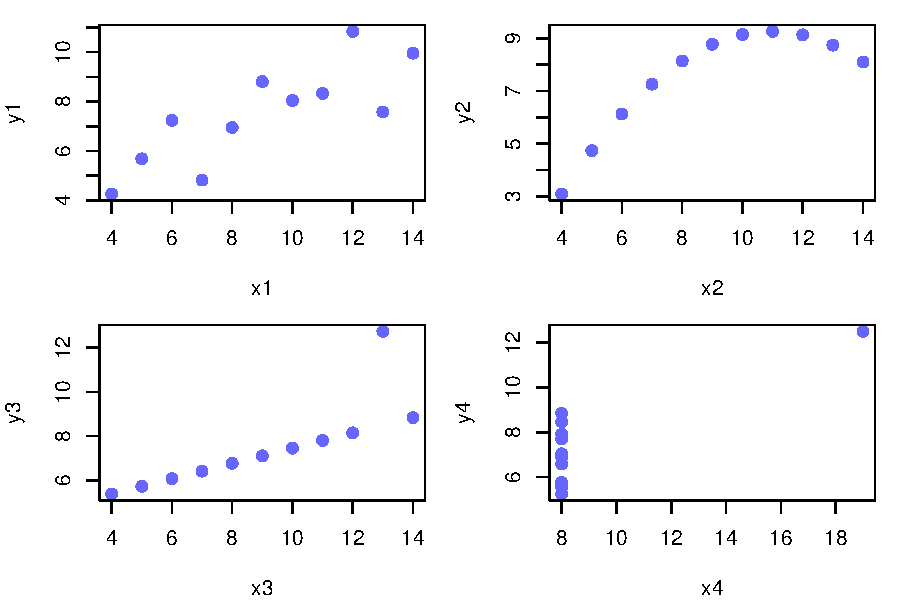
\includegraphics[width=.9\linewidth,height=.7\linewidth]{figure/unnamed-chunk-7-1} 

}



\end{knitrout}

\end{frame}

%------------------------------------------------

\begin{frame}
\frametitle{Data Visualization}

Using only numerical reduction methods in data analyses is far too limiting.

\bigskip
Visualization provides insight that cannot be appreciated by any other approach to learning from data. (W. S. Cleveland)

\end{frame}

%------------------------------------------------

\begin{frame}
\frametitle{Data Visualization}

A key component of computing with data consists of \textbf{Data Visualization}

\bigskip
Google \code{"data visualization"}

\end{frame}

%------------------------------------------------

\begin{frame}
\frametitle{Data Visualization}
\begin{center}
\ig[width=8cm]{images/vis_areas.pdf}
\end{center}
\end{frame}

%------------------------------------------------

\begin{frame}
\frametitle{Data Visualization}

Data Visualization
\bi
  \item Statistical Graphics?
  \item Computer Graphics?
  \item Computer Vision?
  \item Infographics?
  \item Data Art?
\ei

\end{frame}

%------------------------------------------------

\begin{frame}
\frametitle{Infographic}
\begin{center}
\ig[width=9cm]{images/infographic.png}
\end{center}
\end{frame}

%------------------------------------------------

\begin{frame}
\frametitle{Scientific Imaging}
\begin{center}
\ig[width=7cm]{images/imaging.jpg}
\end{center}
\end{frame}

%------------------------------------------------

\begin{frame}
\frametitle{Data Art}
\begin{center}
\ig[width=11cm]{images/windmap.png}
\end{center}
\end{frame}

%------------------------------------------------

\begin{frame}
\frametitle{Visualization Continuum}
\begin{center}
\ig[width=10cm]{images/vis_continuum.pdf}
\end{center}
\end{frame}

%------------------------------------------------

\begin{frame}
\frametitle{Data Art?}

{\large There's value in entertaining, putting a smile on someone's face, and making people feel something, as much as there is in optimized presentation.}

\bigskip
{\footnotesize Nathan Yau, 2013\\
(Data Points, p 69)
}

\end{frame}

%------------------------------------------------

\begin{frame}
\frametitle{Data Art?}

{\large \textbf{Data Art}: visualizations that strive to entertain or to create aesthetic experiences with little concern for informing.}

\bigskip
{\footnotesize Stephen Few, 2012}

\end{frame}

%------------------------------------------------

\begin{frame}
\frametitle{Data Visualization}
\begin{center}
\ig[width=8cm]{images/vis_areas.pdf}
\end{center}
\end{frame}

%------------------------------------------------

\begin{frame}
\frametitle{Stats Graphics}
\begin{center}
\ig[width=8cm]{images/Rgraphics.pdf}
\end{center}
\end{frame}

%------------------------------------------------

\begin{frame}
\frametitle{Stats Graphics}

\bb{Things commonly said about statistical graphics}
\bi
  \item The data should stand out
  \item Story telling
  \item Big Picture
  \item ``The purpose of visualization is insight, not pictures'' (Ben Shneiderman)
\ei
\eb

{\footnotesize We'll focus on statistical graphics and other visual displays of data in science and technology}

\end{frame}

%------------------------------------------------

\begin{frame}
\frametitle{Stats Graphics}

\centerline{\mdlit \Large Graphics for}

\bigskip
\centerline{\Large Exploration \quad \& \quad Communication}

\end{frame}

%------------------------------------------------

\begin{frame}
\frametitle{Graphics for Exploration}

\bbi
  \item graphics for understanding data
  \item the analyst is the main (and usually only) consumer
  \item typically quick \& dirty (not much care about visual appearance and design principles)
  \item lifespan of a few seconds
\ei

\end{frame}

%------------------------------------------------

\begin{frame}
\frametitle{Graphics for Exploration}

\begin{knitrout}\footnotesize
\definecolor{shadecolor}{rgb}{0.969, 0.969, 0.969}\color{fgcolor}

{\centering 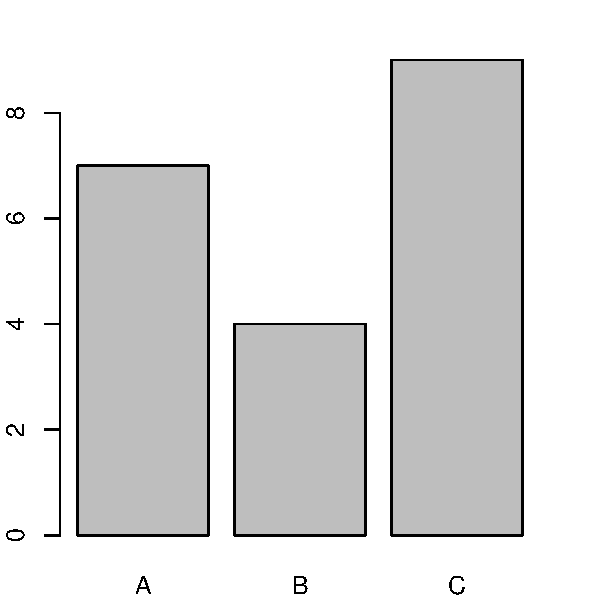
\includegraphics[width=.7\linewidth,height=.6\linewidth]{figure/unnamed-chunk-8-1} 

}



\end{knitrout}

\end{frame}

%------------------------------------------------

\begin{frame}
\frametitle{Graphics for Communication}

\bi
  \item graphics for presenting data
  \item to be consumed by others
  \item must care about visual appearance and design
  \item require a lot of iterations in order to get the final version
  \item what's the message? 
  \item who's the audience?
  \item on what type of media / format?
\ei

\end{frame}

%------------------------------------------------

\begin{frame}
\frametitle{Graphics for Communication}

\begin{knitrout}\footnotesize
\definecolor{shadecolor}{rgb}{0.969, 0.969, 0.969}\color{fgcolor}

{\centering 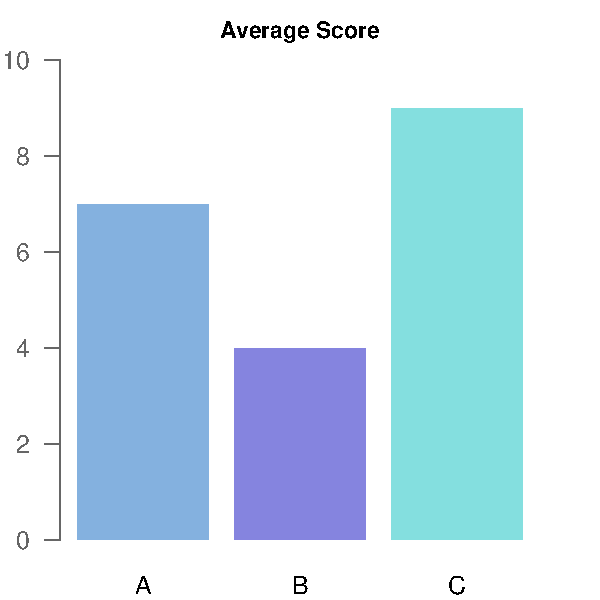
\includegraphics[width=.7\linewidth,height=.6\linewidth]{figure/unnamed-chunk-9-1} 

}



\end{knitrout}

\end{frame}

%------------------------------------------------

\begin{frame}
\frametitle{Graphics for Communication}

Use visualization to communicate ideas, influence, explain persuade

\bigskip
Visuals can serve as evidence or support

\end{frame}

%------------------------------------------------

\begin{frame}
\frametitle{Visualization}

\bbi
  \item Visuals can frequently take the place of many words, tables, and numbers
  \item Visuals can summarize, aggregate, unite, explain
  \item Sometimes words are needed, however
\ei

\end{frame}

%------------------------------------------------

\begin{frame}
\frametitle{Graphics (Part I)}

In this first part of the course we'll focus on:
\bi
  \item graphics for exploration
  \item types of statistical graphics
  \item understanding graphics system in R
  \item traditional R graphics and graphics with \code{"ggplot2"}
\ei

\end{frame}

%------------------------------------------------

\begin{frame}
\frametitle{Graphics (Part II)}

Later in the course we'll talk about:
\bi
  \item graphics for communication
  \item design principles
  \item color theory and use of color
  \item guidelines and good practices
  \item \code{"shiny"} and interactive graphics (time permitting)
\ei

\end{frame}

%------------------------------------------------

\begin{frame}
\frametitle{Considerations}

\centerline{\mdlit \large Number of Variables}

\bigskip
\centerline{\Large \large Type of Variables}

\end{frame}

%------------------------------------------------

\begin{frame}
\frametitle{How many variables?}

Variables in datasets:
\bi
  \item 1 - univariate data
  \item 2 - bivariate data
  \item 3 - trivariate data
  \item multivariate data
\ei

\end{frame}

%------------------------------------------------

\begin{frame}
\frametitle{What type of variables?}

\bbi
  \item Quantitative -vs- Qualitative
  \item Continuous -vs- Discrete
\ei

\end{frame}

%------------------------------------------------

\begin{frame}
\frametitle{Univariate}

Quantitative variable:
\bi
  \item How values are distributed
  \item max, min, ranges
  \item measures of center
  \item measures of spread
  \item areas of concentration
  \item outliers
  \item interesting patterns
\ei

\end{frame}

%------------------------------------------------

\begin{frame}
\frametitle{Univariate}

Qualitative variable:
\bi
  \item Counts and proportions (i.e. frequencies)
  \item Common values
  \item Most typical value
  \item Distribution of frequencies
\ei

\end{frame}

%------------------------------------------------

\begin{frame}
\frametitle{Bivariate}

\bbi
  \item Quantitative-Quantitative
  \item Qualitative-Quantitative
  \item Qualitative-Qualitative
\ei
In general we care about association (correlation, relationships)

\end{frame}

%------------------------------------------------

\begin{frame}
\frametitle{Multivariate}

\bbi
  \item Quantitative
  \item Qualitative
  \item Mixed
\ei
In general we care about association (correlation, relationships)

\end{frame}

%------------------------------------------------

\begin{frame}
\frametitle{What about individuals?}

\bbi
  \item Resemblance
  \item Similarities and disimilarities
  \item Typologies
\ei

\end{frame}

%------------------------------------------------

\end{document}
